\documentclass[a4paper]{scrartcl}
\usepackage[utf8]{inputenc}
\usepackage{graphicx}
\usepackage{lastpage}
\usepackage{pgf}
\usepackage{wrapfig}
\usepackage{fancyvrb}
\usepackage{fancyhdr}
\usepackage{url}
\usepackage{array}
\usepackage{tikz}
\usetikzlibrary{patterns}
% \usetikzlibrary{crypto.symbols}
\pagestyle{fancy}
\setlength{\parindent}{0pt}
\usepackage{mathtools}
\usepackage{tikz}
\usetikzlibrary{shapes}
\usepackage{algorithmicx}
\usepackage[noend]{algpseudocode}
\usepackage{amssymb}
\newcommand{\inv}{^{\raisebox{.2ex}{$\scriptscriptstyle-1$}}}
\newcommand{\ts}{\textsuperscript}
\usepackage{listings}

% Remove hyphenation
\usepackage[british]{babel}
\tolerance=1
\emergencystretch=\maxdimen
\hyphenpenalty=10000
\hbadness=10000
\setlength{\parskip}{0.5cm plus4mm minus3mm}

% Create header and footer
\headheight 27pt
\renewcommand{\headrulewidth}{0.4pt}
\fancyhead[L]{DD2448}
\fancyhead[R]{Phillip Gajland}
\fancyfoot[C]{\thepage\ (\pageref{LastPage})}

% Create title page
\title{Foundations of Cryptography}
\subtitle{Summary of the course DD2448 taught at\\KTH Royal Institute of Technology by Douglas Wikström}
\author{Phillip Gajland}
\date{Spring 2019}

\begin{document}
\thispagestyle{empty}
\maketitle

\section*{Lecture 1 - Introduction \& Symmetric Cryptosystems}

\subsection*{General}

\begin{itemize}
\item Alice encrypts a message $m$ using key $k$ and encryption algorithm $E$ such that $c = E_k(m)$. Bob decrypts the ciphertext $c$ using the same key $k$ and decryption algorithm  $E\inv$ such that $m = E_k\inv(c)$.
\item Mathematically, a cryptosystem can be defined as a tuple $({\mathcal Gen},{\mathcal {P}}, E, E\inv)$ where:
\begin{itemize}
\item [$\circ$] ${\mathcal Gen}$ is a key generation algorithm for keys in the key space ${\mathcal {K}}$.
\item [$\circ$] ${\mathcal {P}}$ is the set of plaintexts.
\item [$\circ$] $E$ is a deterministic encryption algorithm.
\item [$\circ$] $E\inv$ is a deterministic decryption algorithm.
\end{itemize}
such that $E_k\inv(E_k(m)) = m$ for every message $m \in {\mathcal {P}}$ and $k \in {\mathcal {K}}$
\item The set ${\mathcal {C}} = E_k(m) \mid m \in {\mathcal {P}} \land k \in {\mathcal {K}}$ is called the set of ciphertexts.

(Pronounced: \textit{$E_k(m)$ such that $m$ is in ${\mathcal {P}}$ and $k$ is in ${\mathcal {K}}$.} I.e. all combinations of keys $k$ and messages $m$.
\end{itemize}

\subsection*{Caesar Cipher}

\begin{itemize}
\item In an alphabet containing 26 letters, the key $k$ is such that $k \in \mathbb{Z}_{26}$.
\item The plaintext $m = (m_1, ..., m_n) \in \mathbb{Z}_{26}^{n}$ gives ciphertext $c = (c_1, ..., c_n)$.
\item Encryption is given by $c_i = m_i + k \mod 26$.
\item Decryption is given by $m_i = c_i - k \mod 26$.
\item The key space ${\mathcal {K}}$ is too small, making it susceptible to brute force attacks.
\item A frequency analysis can be done by maximising the inner product $T(E\inv(C)) \cdot F$ where $T(s) \cdot F$ denotes the frequency table of string $s$ and the English language respectively.
\end{itemize}

\section*{Lecture 2 - More Symmetric Cryptosystems}

\subsection*{Affine Cipher}

\begin{itemize}
\item The key $k$ is given by a random pair $(a, b)$, where $a \in \mathbb{Z}_{26}$ is relatively prime to 26, and $b \in \mathbb{Z}_{26}$.
\item The plaintext $m = (m_1, ..., m_n) \in \mathbb{Z}_{26}^{n}$ gives ciphertext $c = (c_1, ..., c_n)$.
\item Encryption is given by $c_i = am_i + b \mod 26$.
\item Decryption is given by $m_i = (c_i - b)a^{-1} \mod 26$.
\item \textsl{Relative primality of $a$ and 26 implies that $(a^{-1} \mod 26)$ exists.}
\end{itemize}

\subsection*{Substitution Cipher}

\begin{itemize}
\item Both the Caesar cipher and affine cipher are examples of substitution ciphers.
\item The key is a random permutation $\sigma \in {\mathcal {S}}$ of the symbols in the alphabet, for some subset ${\mathcal {S}}$ of all permutations.
\item The plaintext $m = (m_1, ..., m_n) \in \mathbb{Z}_{26}^{n}$ gives ciphertext $c = (c_1, ..., c_n)$.
\item Encryption is given by $c_i = \sigma(m_i)$.
\item Decryption is given by $m_i = \sigma^{-1}(c_i)$.
\end{itemize}

\subsubsection*{Generic Attacks on Substitution Ciphers}

\begin{itemize}
\item A \textbf{digram} is an ordered pair of symbols.
\item A \textbf{trigram} is an ordered triple of symbols.
\item It is useful to compute frequency tables for the most frequent digrams and trigrams, and not only the frequencies for individual symbols. 

\begin{enumerate}
\item Compute symbol / digram / trigram frequency tables for the candidate language and the ciphertext.
\item Try to match symbols / digrams / trigrams with similar frequencies. 
\item Try to recognise words to confirm guesses (using dictionary or Google).
\item Repeat until the plaintext can be guessed.
\end{enumerate}
\item This is hard when several symbols have similar frequencies - a large amount of cipher text is needed.
\end{itemize}

\subsection*{Vigenère Cipher}

\begin{itemize}
\item The key is given by $k = (k_0, ..., k_{l - 1})$, where $k_i \in \mathbb{Z}_{26}$ is random.
\item The plaintext $m = (m_1, ..., m_n) \in \mathbb{Z}_{26}^{n}$ gives ciphertext $c = (c_1, ..., c_n)$.
\item Encryption is given by $c_i = m_i + k_{i \mod l} \mod 26$.
\item Decryption is given by $m_i = c_i - k_{i \mod l} \mod 26$.
\item \textsl{This gives a more uniform frequency table.}
\end{itemize}

\subsubsection*{Attack on Vigenère Cipher}

\begin{itemize}
\item Each probability distribution $p_1, ..., p_n$ on $n$ symbols may be viewed as a point $p = (p1, ..., p_n)$ on a $n - 1$ dimensional hyperplane in $\mathbb{R}^n$ orthogonal to the vector $\overline{1} = (1, ..., 1)$.
\item Such a point $p = (p_1, ..., p_n)$ is at a distance $\sqrt{F(p)}$ from the origin, where $F(p) = \sum^{n}_{i = 1} p^2_i$.
\item It is clear that $p$ is closest to the origin, when $p$ is the uniform distribution, i.e., when $F(p)$ is minimised.
\item $F(p)$ is invariant under permutation of the underlying symbols. Use tools to check if a set of symbols is the result of some substitution cipher. 
\begin{enumerate}
\item For $l = 1, 2, 3, ...$ we form\\[0.25cm] 
$
\begin{pmatrix}
C_{0} \\
C_{1} \\
\vdots \\
C_{l-1} 
\end{pmatrix} 
=
\begin{pmatrix}
c_{0} & c_{l} & c_{2l} & \cdots \\
c_{1} & c_{l+1} & c_{2l+1} & \cdots \\
\vdots  & \vdots  & \vdots & \ddots \\
c_{l-1} & c_{2l-1} & c_{3l-1} & \cdots 
\end{pmatrix}$\\[0.25cm]
and compute $f_l = \frac{1}{l} \sum^{l-1}_{i=0}F(C_i)$.
\item The local maximum with smallest $l$ is probably the right length.
\item Then attack each $C_i$ separately to recover $k_i$, using the attack against the Caesar cipher.
\end{enumerate}
\end{itemize}

\subsection*{Hill Cipher}

\begin{itemize}
\item The key is given by $k = A$, where $a$ is an invertible $l \times l$-matrix over $\mathbb{Z}_{26}$.
\item The plaintext $m = (m_1, ..., m_n) \in \mathbb{Z}_{26}^{n}$ gives ciphertext $c = (c_1, ..., c_n)$.
\item Encryption is given by $(c_{i+0}, ..., c_{i+l-1}) = (m_{i+0}, ..., m_{i+l-1})A$.
\item Decryption is given by $(c_{i+0}, ..., c_{i+l-1}) = (m_{i+0}, ..., m_{i+l-1})A^{-1}$.\\[0.25cm]
for $i = 1, l + 1, 2l + 1, ...$
\item The Hill cipher is easy to break using a \textbf{known plaintext attack}.
\end{itemize}

\subsection*{Permutation Cipher}

\begin{itemize}
\item The permutation cipher is a special case of the Hill cipher.
\item The key is given by a random permutation $\pi \in \mathcal{S}$ for some subset $\mathcal{S}$ of the set of permutation of $\{0, 1, 2, ..., l -1\}$.
\item The plaintext $m = (m_1, ..., m_n) \in \mathbb{Z}_{26}^{n}$ gives ciphertext $c = (c_1, ..., c_n)$.
\item Encryption is given by $c_i = m_{\lfloor i / l \rfloor + \pi (i \mod l)}$.
\item Decryption is given by $m_i = c_{\lfloor i / l \rfloor + \pi^{-1} (i \mod l)}$.
\end{itemize}

\subsection*{Summary of Simple Ciphers}

\begin{itemize}
\item Caesar cipher and affine cipher: $m_i \mapsto am_i + b$.
\item Substitution cipher (generalise Caesar / affine): $m_i \mapsto \sigma(m_i)$.
\item Vigenère cipher (more uniform frequency table): $m_i \mapsto m_i + k_{i \mod l}$.
\item Hill cipher (invertible linear map): $(m_1, ..., m_l) \mapsto (m_1, ..., ..., m_l)A$.
\item Transposition cipher (permutation): $(m_1, ..., m_l) \mapsto (m_{\pi(1)}, ..., m_{\pi(l)})$\\
equivalent to: $(m_1, ..., m_l) \mapsto (m_1, ..., m_l)M_\pi$.
\end{itemize}

\subsection*{Good Block Ciphers}

\begin{itemize}
\item Simple ciphers are bad, but what makes a good block cipher?
\item For every key a block-cipher with plaintext / ciphertext space $\{0, 1\}^n$ gives a permutation of $\{0, 1\}^n$.
\begin{itemize}
\item [$\circ$] What would be a good cipher?
\end{itemize}
\item A good cipher is one where each key gives a \textbf{randomly chosen permutation} of $\{0, 1\}^n$.
\begin{itemize}
\item [$\circ$] Why is this not possible?
\end{itemize}
\item The representation of a single typical function $\{0, 1\}^n \rightarrow \{0, 1\}^n$ requires roughly $n2^n$ bits $(147 \times 10^{6 \cdot 3}$ for $n = 64)$.
\begin{itemize}
\item [$\circ$] What should we look for instead?
\end{itemize}
\item \textbf{Idea:} Compose smaller weak ciphers into a large one. Mix the components thoroughly. Claude Shannon (1948) introduces two terms:
\begin{itemize}
\item [$\circ$] \textbf{Diffusion:} "In the method of diffusion the statistical structure of $M$ which leads to its redundancy is dissipated into long range statistics..."
\item [$\circ$] \textbf{Confusion:} "The method of confusion is to make the relation between the simple statistics of $E$ and the simple description of $K$ a very complex and involved one."
\end{itemize}
\end{itemize}

\section*{Lecture 3 - Substitution-Permutation Networks \& AES}

\subsection*{Substitution-Permutation Networks}

\begin{itemize}
\item Block-size: We use a block-size of $n = l \times m$ bits.
\item Key Schedule: Round $r$ uses its own round key $K_r$ derived from the key $K$ using a key schedule.
\item Each Round the following is invoked:
\begin{enumerate}
\item Round Key: xor with the round key.
\item Substitution: $l$ substitution boxes each acting on one $m$-bit word ($m$-bit S-Boxes).
\item Permutation: A permutation $\pi_i$ acting on $\{1, ..., n\}$ to reorder the $n$ bits.
\end{enumerate}
\end{itemize}

\subsection*{A Simple Block Cipher}

\begin{itemize}
\item $|P| = |C| = 16$
\item 4 rounds
\item $|K| = 32$
\item $r$\ts{th} round key $K_r$ consists of the 4$r$\ts{th} to the $(4r + 16)$\ts{th} bits of key $K$.
\item 4-bit S-Boxes
\item S-Boxes the same $(S \neq S\inv)$
\item $Y = S(X)$
\item Can be described using 4 boolean functions.
\end{itemize}

\subsection*{Advanced Encryption Standard (AES)}

\begin{itemize}
\item Chosen in worldwide public competition 1997-2000. Probably no backdoors. Increased confidence!
\item Winning proposal named "Rijndael", by Rijmen and Daemen.
\item Family of 128-bit ciphers: \{Key bits, Rounds\} - \{128, 10\}, \{192, 12\}, \{256, 14\}. 
\item The first key-recovery attacks on full AES found by Bogdanov, Khovratovich, and Rechberger was published in 2011 and is faster than brute force by a factor of about 4. 
\item The algebraics of AES have made some people \textit{uneasy}, but they have been uneasy for years now...
\begin{itemize}
\item [$\circ$] AddRoundKey: xor with round key.
\item [$\circ$] SubBytes: Substitution of bytes.
\item [$\circ$] ShiftRows: Permutation of bytes.
\item [$\circ$] MixXolumns: Linear map.
\end{itemize}
\end{itemize}

\begin{itemize}
\item The 128 bit state is interpreted as a $4 \times 4$ matrix of bytes.
\begin{center}
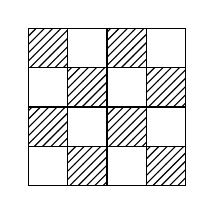
\begin{tikzpicture}[scale=0.5]
\fill[pattern=north east lines] (0,3) rectangle +(1,1);
\fill[pattern=north east lines] (1,2) rectangle +(1,1);
\fill[pattern=north east lines] (2,1) rectangle +(1,1);
\fill[pattern=north east lines] (3,0) rectangle +(1,1);
\fill[pattern=north east lines] (2,3) rectangle +(1,1);
\fill[pattern=north east lines] (3,2) rectangle +(1,1);
\fill[pattern=north east lines] (0,1) rectangle +(1,1);
\fill[pattern=north east lines] (1,0) rectangle +(1,1);
\draw (0,0) rectangle (4,4);
\draw (0,1) -- +(4,0);
\draw (0,2) -- +(4,0);
\draw (0,3) -- +(4,0);
\draw (1,0) -- +(0,4);
\draw (2,0) -- +(0,4);
\draw (3,0) -- +(0,4);
\end{tikzpicture}
\end{center}
\item Something like a mix between substitution, permutation, affine version of Hill cipher. In each round!
\item SubBytes is a field inversion in $\mathbb{F}_{2^8}$ plus affine map in $\mathbb{F}_{2}^8$.
\item ShiftRows is ac cyclic shift of bytes with offsets: 0, 1, 2, and 3.
\item MixColumns is an invertible linear map over $\mathbb{F}_{2^8}$ (with irreducible polynomial $x^8 + x^4 +x^3 + x + 1)$ with good diffusion. 
\item Decryption uses the following transforms:
\begin{itemize}
\item [$\circ$] AddRoundKey
\item [$\circ$] InvSubBytes
\item [$\circ$] InvShiftRows
\item [$\circ$] InvMixColumns
\end{itemize}
\end{itemize}

\subsection*{Feistel Networks}

\begin{itemize}
\item Identical rounds are iterated, but with different round keys.
\item The input to the $i$\ts{th} round is divided in a left and right part, denoted $L^{i-1}$ and $R^{i-1}$.
\item $f$ is a function for which it is somewhat hard to find pre-images, but $f$ is \textbf{not invertible}!
\item One round is defined by:\\ 
$L^i = R^{i-1}$\\$R^i = L^{i-1} \oplus f(R^{i-1}, K^i)$\\
where $K^i$ is the $i$\ts{th} round key.
\item The inverse Feistel round is given by:\\ 
$L^{i-1} = R^i \oplus f(L^i, K^i)$\\$R^{i-1} = L^i$\\
I.e. reverse direction and swap left and right.
\end{itemize}

\subsection*{Data Encryption Standard (DES)}
\begin{itemize}
\item Developed at IBM in 1975, or perhaps at NSA; not publicly known.
\item 16-round Feistel network.
\item Key schedule derives permuted bits for each round key from a 56-bit key. Supposedly not 64-bit due to parity bits.
\item DES's $f$-Function is given by: $f(R^{i-1}, K^i)$
\end{itemize}

\subsection*{Security of DES}
\begin{itemize}
\item Brute Force: Try all $2^56$ keys. Done in practice with special chip by Electronic Frontier Foundation, 1998. Possibly much earlier by NSA and others.
\item Differential Cryptanalysis: $2^{47}$ chosen plaintexts, Biham and Shamir, 1991. Known earlier by IBM and NSA. DES is surprisingly resistant!
\item Linear Cryptanalysis: $2^{43}$ known plaintexts, Matsui, 1993. Probably \textbf{not} known by IBM and NSA!
\item Since the key space for DES is too small, one way to increase it is to use DES twice, so called "double DES".
$2DES_{k_1,k_2}(x) = DES_{k_2}(DES_{k_1}(x))$.
\item However, this is \textbf{not} more secure than normal DES! 
\item Meet-in-the-middle attack:
\begin{itemize}
\item [$\circ$] Get hold of a plaintext-ciphertext pair $(m, c)$.
\item [$\circ$] Compute $X = \{x \mid k_1 \in \mathcal{K}_{DES} \land x = E_{k_1}(m) \}$.
\item [$\circ$] For $k_2 \in \mathcal{K}_{DES}$ check if $E_{k_2}^{-1}(c) = E_{k_1}(m)$ for some $k_1$ using the table $X$. If so, then $(k_1, k_2)$ is a good candidate.
\item [$\circ$] Repeat with $(m', c')$, starting from the set of candidate keys to identify the correct key.
\end{itemize}
\item Tripple DES: $3DES_{k_1,k_2,k_3}(x) = DES_{k_3}(DES_{k_2}(DES_{k_1}(x)))$.
\item Seemingly 112 bit "effective" key size.
\item 3 times as slow as DES. DES is slow in software, and this is even worse. One of the motivation for AES. 
\item Triple DES is sill considered to be secure.
\end{itemize}

\subsection*{Modes of Operation}
\begin{itemize}
\item 5 modes of operation:
\begin{itemize}
\item [$\circ$] Electronic codebook mode (ECB mode).
\item [$\circ$] Cipher feedback mode (CFB mode).
\item [$\circ$] Cipher block chaining mode (CBC mode).
\item [$\circ$] Output feedback mode (OFB mode).
\item [$\circ$] Counter mode (CTR mode).
\end{itemize}
\item \textbf{Electronic codebook mode} - encrypt each block independently: $c_i = E_k(m_i)$.
\item Identical plaintext blocks give identical ciphertext blocks.
\item \textbf{Cipher feedback mode} - xor plaintext block with previous ciphertext block \textbf{after} encryption:\\$c_0 =$ initialisation vector\\$c_i = m_i \oplus E_k(c_{i-1})$.
\item Sequential encryption and parallel decryption.
\item Self-synchronising and unidirectional.
\item \textbf{Cipher block chaining mode} - xor plaintext block with previous ciphertext block \textbf{after} encryption:\\$c_0 =$ initialisation vector\\$c_i = E_k(c_{i-1} \oplus m_i)$.
\item Sequential encryption and parallel decryption.
\item Self-synchronising.
\item \textbf{Output feedback mode} - generate stream, xor plaintexts with stream (emulate "one-time pad"):\\$s_0 =$ initialisation vector\\$s_i = E_k(s_{i-1})$\\$c_i = s_i \oplus m_i$.
\item Sequential. 
\item Synchronous.
\item Allows batch processing.
\item Malleable!
\item \textbf{Counter mode} - generate stream, xor plaintexts with stream (emulate "one-time pad"):\\$s_0 =$ initialisation vector\\$s_i = E_k(s_{0} || i)$\\$c_i = s_i \oplus m_i$.
\item Parallel.
\item Synchronous.
\item allows batch processing.
\item Malleable!
\end{itemize}

\section*{Lecture 4 - Cryptanalysis of the Simple Permutation Network}

\begin{itemize}
\item Find an expression of the following form with a high probability of occurrence. 
$$P_{i_1} \oplus \cdots \oplus P_{i_p} \oplus C_{j_1} \oplus \cdots \oplus C_{j_c} = K_{l_1, s_1} \oplus \cdots \oplus K_{l_k, s_k}$$
\item Each random plaintext / ciphertext pair gives an estimate of $$K_{l_1, s_1} \oplus \cdots \oplus K_{l_k, s_k}$$
\item Collect many pairs and make a better estimate based on the majority vote.
\item How do we come up with the desired expression?
\item How do we compute the required number of samples?
\end{itemize}
\subsection*{Bias}
\begin{itemize}
\item The bias $\epsilon(X)$ of a binary random variable $X$ is defined by $$\epsilon(X) = Pr [X = 0] - \frac{1}{2}$$
$\approx 1 / \epsilon^2(X)$ samples are required to estimate $X$.
\end{itemize}

\subsection*{Linear Approximation of S-Box}
\begin{itemize}
\item Let $X$ and $Y$ be the input and output of an $S$-box, i.e. {\boldmath$Y = S(X)$}.
\item We consider the bias of linear combinations of the form $$a \cdot X \oplus b \cdot Y = \Bigg(\bigoplus_{i}a_iX_i\Bigg) \oplus \Bigg(\bigoplus_{i}b_iY_i\Bigg)$$
\item Example: $X_2 \oplus X_3 = Y_1 \oplus Y_3 \oplus Y_4$. The expression holds in 12 out of the 16 cases. Hence, it has a bias of (12-8)/16 = 4/16 = 1/4.
\item Let $N_L(a, b)$ be the number of zero-outcomes of a $a \cdot X \oplus b \cdot Y$.
\item The bias is then $$\epsilon(a \cdot X \oplus b \cdot Y = \frac{N_L(a,b) - 8}{16},$$ since there are four bits in $X$, and $Y$ is determined by $X$.
\item This gives a linear approximation for one round.
\item How do we come up with a linear approximation for more rounds?
\end{itemize}

\subsection*{Piling-Up Lemma}

\begin{itemize}
\item Let $X1, ..., X_t$ be independent binary random variables and let $\epsilon_i = \epsilon(X_i)$. Then $$\epsilon \Bigg(\bigoplus_{i}X_i\Bigg) = 2^{t-1} \prod_{i} \epsilon_i .$$ 
\item Proof: Case $t = 2$:
\begin{align*}
Pr[X_1 \oplus X_2 = 0] &= Pr[X_1 = 0 \land X_1 = 0) \lor (X_1 = 1 \land X_1 = 1)]\\
&= (\frac{1}{2} + \epsilon_1)(\frac{1}{2} + \epsilon_2)+(\frac{1}{2} - \epsilon_1)(\frac{1}{2} - \epsilon_2)\\
&=\frac{1}{2} + 2\epsilon_1 \epsilon_2.
\end{align*}
By induction $Pr[X_1 \oplus \cdots \oplus X_t = 0] = \frac{1}{2} + 2^{t-1}\prod_{i} \epsilon_i$
\end{itemize}
\subsection*{Attacking a Linear Trail}
\begin{itemize}
\item Four linear approximations with $|\epsilon_i| = 1/4$
\begin{align*}
S_{12} &: X_1 \oplus X_3 \oplus X_4 = Y_2\\
S_{22} &: X_2 = Y_2 \oplus Y_4\\
S_{32} &: X_2 = Y_2 \oplus Y_4\\
S_{24} &: X_2 = Y_2 \oplus Y_4
\end{align*}
Combine them to get:
$$U_{4,6} \oplus U_{4,8} \oplus U_{4,14} \oplus U_{4,16} \oplus P_5 \oplus P_7 \oplus P_8 = \bigoplus K_{i,j}$$
with bias $|\epsilon| = 2^{4-1}(\frac{1}{4})^4 = 2^{-5}$
\item Our expression (with bias $2^{-5}$) links plaintext bits to input bits to the 4\ts{th} round.
\item Partially undo the last round by guessing the last key. Only 2 S-Boxes are involved, i.e., $2^8 = 256$ guesses.
\item For a correct guess, the question holds with bias $2^{-5}$. For a wrong guess, it holds with a bias zero (harmless lie).
\item Required pairs $2^{10} \approx 1000$. Attack complexity $2^{18} \ll 2^{32}$ operations.
\end{itemize}

\subsection*{Linear Cryptanalysis Summary}
\begin{itemize}
\item Linear Cryptanalysis is a \textbf{known plaintext attack}.
\begin{itemize}
\item [$\circ$] Find linear approximation of S-Boxes.
\item [$\circ$] Compute bias of each approximation.
\item [$\circ$] Find linear trails.
\item [$\circ$] Compute bias of linear trails.
\item [$\circ$] Compute data and time complexity.
\item [$\circ$] Estimate key bits from many plaintext-ciphertext pairs.
\end{itemize}
\end{itemize}

\subsection*{Ideal Block Cipher}

\begin{itemize}
\item A function $\epsilon(n)$ is negligible if for every constant $c > 0$, there exists a constant $n_0$, such that $$\epsilon(n) < \frac{1}{n^c}$$ for all $n \geq n_0$.
\item Motivation: Events happening with negligible probability can not be exploited by polynomial time algorithms! (they "never" happen!)
\item Caveat! Theoretic notion. Interpret with care in practice.
\item A function is pseudo-random if no efficient adversary can distinguish between the function and a random function.
\item A family of functions $F: \{0,1\}^k \times \{0,1\}^n \rightarrow \{0,1\}^n$ is pseudo-random if for all polynomial time oracle adversaries $A$
$$\Bigg|\Pr_{K} \Big[A^{F_K(\cdot)}=1 \Big] - \Pr_{R:\{0,1\}^n \rightarrow \{0,1\}^n} \Big[A^{R(\cdot)}=1\Big] \Bigg|$$ is negligible.
\item A permutation and its inverse are pseudo-random if no efficient adversary can distinguish between the permutation and its inverse, and a random permutation and its inverse.
\item A family of permutations $P: \{0,1\}^k \times \{0,1\}^n \rightarrow \{0,1\}^n$ is pseudo-random if for all polynomial time oracle adversaries $A$
$$\Bigg|\Pr_{K} \Big[A^{P_K(\cdot),P_K^{-1}(\cdot)}=1 \Big] - \Pr_{\Pi \in {\mathcal S}_{2^n}} \Big[A^{\Pi(\cdot),\Pi^{-1}(\cdot)}=1\Big] \Bigg|$$ 
is negligible, where ${\mathcal S}_{2^n}$ is the set of permutations of $\{0,1\}^n$.
\end{itemize}

\subsection*{Idealised Four-Round Feistel Network}

\begin{itemize}
\item Feistel round ($H$ for "Horst Feistel").
$$H_{F_K}(L,R) = (R, L \oplus F(R,K))$$
\item Theorem: (Luby and Rackoff) If $F$ is a pseudo-random family of functions, then
$$H_{F_{k_1},F_{k_2},F_{k_3},F_{k_4}}(x) = H_{F_{k_4}}(H_{F_{k_3}}(H_{F_{k_2}}(H_{F_{k_1}}(x))))$$ (and its inverse) is a pseudo-random family of permutations.
\item Why do we need four rounds?
\end{itemize}

\subsection*{Perfect Secrecy}
\begin{itemize}
\item When is a cipher perfectly secure?
\item How should we formalise this?
\item A cryptosystem has perfect secrecy if guessing the plaintext is equally hard to do regardless of whether or not the ciphertext is given.
\item A cryptosystem has perfect secrecy if $$Pr[M = m \mid C = c] = Pr[M = m]$$ for every $m \in {\mathcal M}$ and $c \in {\mathcal C}$, where $M$ and $C$ are random variables taking values over ${\mathcal M}$ and ${\mathcal C}$.
\item Game Based Definition: $Exp_A^b$, where $A$ is a strategy:
\begin{itemize}
\item [$\circ$] $k \leftarrow_R {\mathcal K}$
\item [$\circ$] $(m_0, m_1) \leftarrow A$
\item [$\circ$] $c = E_k(m_b)$
\item [$\circ$] $d\leftarrow A(c)$, with $d \in \{0,1\}$
\item [$\circ$] Output $d$.
\end{itemize}
\item A cryptossystem has perfect secrecy if for every computationally unbounded strategy $A$, $$Pr[Exp_A^0 = 1] = Pr[Exp^1_A = 1].$$
\end{itemize}

\subsection*{One-Time Pad (OTP)}
\begin{itemize}
\item The key is given by a random tuple $k = (b_0, ..., b_{n-1}) \in \mathbb{Z}_{2}^{n}$.
\item The plaintext $m = (m_0, ..., m_{n-1}) \in \mathbb{Z}_{2}^{n}$ gives ciphertext $c = (c_0, ..., c_{n-1})$.
\item Encryption is given by $c_i = m_i \oplus b_i$.
\item Decryption is given by $m_i = c_i \oplus b_i$.
\end{itemize}

\subsection*{Bayes' Theorem and OTP's Perfect Secrecy}
\begin{itemize}
\item If $A$ and $B$ are events and $Pr[B] > 0$, then $$Pr[A \mid B] = \frac{Pr[A]Pr[B \mid A]}{Pr[B]}$$
\item Probabilistic Argument. Bayes implies that:
\begin{align*}
Pr[M = m \mid C = c] &= \frac{Pr[M = m]Pr[C = c \mid M = m]}{Pr[C=c]}\\
&=Pr[M = m]\frac{2^{-n}}{2^{-n}}\\
&=Pr[M=m].
\end{align*}
\item Simulation Argument: The ciphertext is uniformly and independently distributed form the plaintext. We can simulate it on our own!
\item Bad News! "For every cipher with perfect secrecy, the key requires at least as much space to represent as the plaintext."
\begin{itemize}
\item [$\circ$] Dangerous in practice to rely on no reuse of, e.g., file containing randomness!
\end{itemize}
\end{itemize}

\section*{Lecture 5 - Hash Functions \& Random Oracles}

\subsection*{Universal Hash Functions}

\begin{itemize}
\item An ensemble $f = \{f_\alpha\}$ of hash functions $f_\alpha : X \rightarrow Y$ is (strongly) 2-universal if for every $x, x' \in X$ and $y, y' \in Y$ with $x \neq x'$ and a random $\alpha$
$$Pr[f_\alpha(x) = y \land f_\alpha(x') = y'] = \frac{1}{|Y|^2} .$$
I.e., for any fixed $x' \neq x$, the outputs $f_\alpha(x)$ and $f_\alpha(x')$ are uniformly and independently distributed when $\alpha$ is chosen randomly.

In particular $x$ and $x'$ are both mapped to the same value with probability $\frac{1}{|Y|}$.
\item Example: The function $f: \mathbb{Z}_p \rightarrow \mathbb{Z}_p$ for prime $p$ defined by $$f(z) = az + b \mod p$$ is strongly 2-universal
\item Proof: Let $x, x', y, y' \in \mathbb{Z}_p$ with $x \neq x'$. Then 
$$
\begin{pmatrix}
x & 1 \\
x' & 1
\end{pmatrix}
\begin{pmatrix}
z_1 \\
z_2
\end{pmatrix}
=
\begin{pmatrix}
y \\
y'
\end{pmatrix}
$$
has a unique solution. Random $(a,b)$ satisfies this solution with probability $\frac{1}{p^2}$.
\item Universal hash functions are \textbf{not} one-way or collision resistant!
\end{itemize}

\subsection*{Hash Functions}
\begin{itemize}
\item A hash function maps arbitrary long bit strings into strings of fixed length.
\item The output of a hash function should be "unpredictable"
\item The following properties should be met by a hash function:
\begin{itemize}
\item [$\circ$] Finding a pre-image of an output should be hard.
\item [$\circ$] Finding two inputs giving the same output should be hard.
\item [$\circ$] The output of the function should be "random".
\end{itemize}
\item Let $f: \{0,1\}^* \rightarrow \{0,1\}$ be a polynomial time commutable function.
\item We can derive an ensemble $\{f_n\}_{n \in \mathbb{N}}$, with $$f_n: \{0,1\}^n \rightarrow \{0,1\}^*$$ by setting $f_n(x) = f(x)$.
\item Note that we may recover $f$ form the ensemble by $f(x) = f_{|x|}(x)$.
\item When convenient we give definitions for a function, but it can be turned into a definition for an ensemble.
\item Consider $F=\{f_n\}_{n \in \mathbb{N}}$, where $f_n$ is itself an ensemble $\{f_{n,\alpha_n}\}_{\alpha_n \in \{0,1\}^n}$, with $$f_{n,\alpha_n}:\{0,1\}^{l(n)} \rightarrow \{0,1\}^{l'(n)}$$ for some length polynomials $l(n)$ and $l'(n)$.
\item Here $n$ is the security parameter and $\alpha_n$ is a "key" that is chosen randomly.
\item We may also view $F$ as an ensemble $\{f_\alpha\}$, where $f_\alpha = \{f_{n,\alpha_n}\}_{n \in \mathbb{N}}$ and $\alpha = \{\alpha_n\}_{n \in \mathbb{N}}$.
\item These conventions allow us to talk about what in everyday language is a "function" $f$ in several convenient ways.
\item FROM NOW ON WE CAN FORGET THE ABOVE AND ASSUME EVERYTHING WORKS....
\end{itemize}

\subsection*{One-Wayness}
\begin{itemize}
\item Definition: A function $f: \{0,1\}^* \rightarrow \{0,1\}^*$ is said to be one-way if for every polynomial time algorithm $A$ and a random $x$ $$Pr[A(f(x)) = x' \land f(x') = f(x)] < \epsilon(n)$$ for a negligible function $\epsilon$.
\item Normally $f$ is computable in polynomial time in its input size.
\item Definition: A function $h: \{0,1\}^* \rightarrow \{0,1\}^*$ is said to be second pre-image resistant if for every polynomial time algorithm $A$ and a random $x$ $$Pr[A(x) = x' \land x' \neq x \land f(x') = f(x)] < \epsilon(n)$$ for a negligible function $\epsilon$.
\item Note that $A$ is given not only the output of $f$, but also the input $x$, but it must find a second pre-image.
\item Definition: Let $f = \{f_\alpha\}_\alpha$ be an ensemble of functions. the "function" $f$ is said to be collision resistant if for every polynomial time algorithm $A$ and randomly chosen $\alpha$ $$Pr[A(\alpha) = (x,x') \land x \neq x' \land f_\alpha(x') = f_\alpha(x)] < \epsilon(n)$$ for a negligible function $\epsilon$.
\item An algorithm that gets a small "advice string" for each security parameter can easily hardcode a collision for a fixed function $f$, which explains the random index $\alpha$.
\end{itemize}

\subsection*{Relations for Compressing Hash Functions}
\begin{itemize}
\item If a function is not second pre-image resistant, then it is not collision-resistant.
\begin{itemize}
\item [$\circ$] Pick random $x$.
\item [$\circ$] Request second pre-image $x' \neq x$ with $f(x') = f(x)$.
\item [$\circ$] Output $x'$ and $x$.
\end{itemize}
\item If a function is not one-way, then it is not second pre-image resistant.
\begin{itemize}
\item [$\circ$] Given a random $x$, compute $y = f(x)$.
\item [$\circ$] Request pre-image $x'$ of $y$.
\item [$\circ$] Repeat until $x' \neq x$, and output $x'$.
\end{itemize}
\end{itemize}

\subsection*{Random Oracles}

\begin{itemize}
\item A random oracle is simply a randomly chosen function with appropriate domain and range.
\item A random oracle is the perfect hash function. Every input is mapped independently and uniformly in the range.
\item Let us consider how a random oracle behaves with respect to our notions of security of hash functions.
\end{itemize}

\subsection*{Pre-Image of Random Oracle}

\begin{itemize}
\item We assume with little loss that an adversary always "knows" if it has found a pre-image, i.e., it queries the random oracle on its output. 
\item Theorem: Let $H: X \rightarrow Y$ be a randomly chosen function and let $x \in X$ be randomly chosen. Then for every algorithm $A$ making $q$ oracle queries
$$Pr[A^{H(\cdot)}(H(x)) = x' \land H(x) = H(x')] \leq 1 - \bigg(1 - \frac{1}{|Y|} \bigg)^q .$$
\item Proof: Each query $x'$ satisfies $H(x') \neq H(x)$ independently with probability $1 = \frac{1}{|Y|}$.
\end{itemize}

\subsection*{Second Pre-Image of Random Oracle}

\begin{itemize}
\item We assume with loss that an adversary always "knows" if it has found a second pre-image, i.e., it quries the random oracle on the input and its output.
\item Theorem: Let $H: X \rightarrow Y$ be a randomly chosen function and let $x \in X$ be randomly chosen. Then for every such algorithm $A$ making $q$ oracle queries
$$Pr[A^{H(\cdot)}(x) = x' \land x \neq x' \land H(x) = H(x')] \leq 1 - \bigg(1 - \frac{1}{|Y|} \bigg)^{q-1} .$$
\item Proof: Same as pre-image case, except we must waste one query on the input value to get the target in $Y$.
\end{itemize}

\subsubsection*{Collision Resistance of Random Oracles}

\begin{itemize}
\item We assume with little loss that and adversary always "knows" if it has found a collision, i.e. it queries the random oracle on its outputs.
\item Theorem: Let $H: X \rightarrow Y$ be a randomly chosen function and let $x \in X$ be randomly chosen. Then for every such algorithm $A$ making $q$ oracle queries
$$Pr[A^{H(\cdot)} = (x, x') \land x \neq x' \land H(x) = H(x')] \leq 1 - \prod_{i=1}^{q-1} \bigg(1 - \frac{i}{|Y|} \bigg)$$

$$Pr[A^{H(\cdot)} = (x, x') \land x \neq x' \land H(x) = H(x')] \leq \frac{q(q-1)}{2|Y|} .$$

\item Proof: $1 - \frac{i-1}{|Y|}$ bounds the probability that the $i\ts{th}$ query does not give a collision for any of the $i-1$ previous queries, conditioned on no previous collisions. 
\end{itemize}

\section*{Lecture 6 - Hash Functions and MACs}

\subsection*{Iterated Hash Functions (Merkle-Damg\aa rd)}

\begin{itemize}
\item Suppose that we are given a collision resistant hash function $$f: \{0,1\}^{n+t} \rightarrow \{0,1\}^n.$$
\item How can we construct a collision resistant hash function $$f: \{0,1\}^* \rightarrow \{0,1\}^n$$ mapping any length inputs?
\item Construction:
\begin{itemize}
\item [$\circ$] Let $x=(x_1, ..., x_k)$ with $|x_i| = t$ and $0<|x_k| \leq t$.
\item [$\circ$] Let $x_{k+1}$ be the total number of bits in $x$.
\item [$\circ$] Pad $x_k$ with zeros until it has length $t$.
\item [$\circ$] $y_0 = 0^n, y_i= f(y_{i-1}, x_i)$ for $i = 1,..., k+1$.
\item [$\circ$] Output $y_{k+1}$
\end{itemize}
\item Here the total number of bits is bounded by $2^t-1$, but this can be relaxed.
\item Suppose $A$ finds collisions in Merkle-Damg\aa rd.
\begin{itemize}
\item [$\circ$] If the number of bits differ in a collision, then we can derive a collision from the last invocation of $f$.
\item [$\circ$] If not, then we move backwards until we get a collision. Since both inputs have the same length, we are guaranteed to find a collision.
\end{itemize}
\end{itemize}

\subsection*{Standardised Hash Functions}

\begin{itemize}
\item Despite that theory says it is impossible, in practice people simply live with \textbf{fixed} hash functions and use them as if they are randomly chosen functions. 
\item \textbf{SHA}
\begin{itemize}
\item [$\circ$] Secure Hash Algorithm (SHA-0,1, and the SHA-2 family) are hash functions standardised by NIST to be used in, e.g., signature schemes and random number generation. 
\item [$\circ$] SHA-0 was weak and withdraws by NIST. SHA-1 was withdrawn 2010. The SHA-2 family is based on similar ideas but seems safe so far.
\item [$\circ$] All are iterated hash functions, starting from a basic compression function.
\end{itemize}
\item \textbf{SHA-3}
\begin{itemize}
\item [$\circ$] NIST ran an open competition for the next hash function, named SHA-3. Several groups of famous researchers submitted proposals. 
\item [$\circ$] Call for SHA-3 explicitly asked for "different" hash functions. 
\item [$\circ$] The competition ended on October 2, 2012, and the hash function Keccak was selected as the winner.
\item [$\circ$] It was constructed by Guido Bertoni, Joan Daemen, Micha\"el Peeters, and Gilles Van Assche.
\end{itemize}
\end{itemize}

\subsection*{Message Authentication Codes (MACs)}

\begin{itemize}
\item Message Authentication Codes (MACs) are used to ensure integrity and authentication of messages.
\item Scenario:
\begin{itemize}
\item [$\circ$] Alice and Bob share a common key $k$.
\item [$\circ$] Alice computes an authentication tag $\alpha = MAC_k(m)$ and sends $(m,\alpha)$ to Bob.
\item [$\circ$] Bob receives $(m',\alpha')$ form Alice, but before accepting $m'$ as coming from Alice, Bob checks that $MAC_k(m')=\alpha'$.
\end{itemize}
\end{itemize}

\subsubsection*{Security of a MAC}
\begin{itemize}
\item A message authentication code MAC is secure if for a random key $k$ and every polynomial time algorithm $A$,
$$Pr[A^{MAC_k(\cdot)}=(m,\alpha) \land MAC_k(m) = \alpha \land \forall i : m \neq m_i]$$
is negligible, where $m_i$ is the $i$\ts{th} query to the oracle $MAC_k(\cdot)$.
\end{itemize}

\subsubsection*{Random Oracle As MAC}

\begin{itemize}
\item Suppose that $H: \{0,1\}^* \rightarrow \{0,1\}^n$ is a random oracle.
\item Then we can construct a MAC as $MAC_k(m) = H(k,m)$.
\item Could we plug in an iterated hash function in place of the random oracle?
\end{itemize}

\subsection*{HMAC}

\begin{itemize}
\item Let $H: \{0,1\}^* \rightarrow \{0,1\}^n$ be a "cryptographic hashfunction", e.g. SHA-256.
\item $HMAC_{k_1, k_2}(x) = H\big(k_2||H(k_1||x)\big)$
\item This is provably secure under the assumption that
\begin{itemize}
\item [$\circ$] $H(k_1||\cdot)$ is unknown-key collision resistant, and
\item [$\circ$] $H(k_2||\cdot)$ is a secure MAC for fixed-size messages.
\end{itemize}
\end{itemize}

\section*{MACs and Information Theory}

\subsection*{MACs}

\subsubsection*{CBC-MAC}

\begin{itemize}
\item Let $E$ be a secure block-cipher, and $x = (x_1,...,x_t)$ an input. The MAC-key is simply the block-cipher key.
\begin{itemize}
\item [$\circ$] $y_0 = 000...0$
\item [$\circ$] For $i=1,...,t$, $y_i = E_k(y_{i-1}\oplus x_i)$
\item [$\circ$] Return $y_t$.
\end{itemize}
\item Is this secure?
\end{itemize}

\subsubsection*{Universal Hashfunction As MAC}
\begin{itemize}
\item Theorem: A $t$-universal hashfunction $f_\alpha$ for a randomly chosen secret $\alpha$ is an \textbf{unconditionally secure} MAC, provided that the number of queries is smaller than $t$.
\end{itemize}

\subsection*{Information Theory}

\begin{itemize}
\item Information theory is a mathematical theory of communication.
\item Typical questions studied are how to compress, transmit, and store information.
\item Information theory is also useful to argue about some cryptographic schemes and protocols.
\item Memory Source Over Finite Alphabet: A source produces symbols from an alphabet $\Sigma = \{a_1,...,a_n\}$. Each generated symbol is independently distributed.
\item Binary Channel: A binary channel can (only) send bits. \item Coder/Decoder: Our goal is to come up with a scheme to:
\begin{itemize}
\item [$\circ$] Convert a symbol $a$ from the alphabet $\Sigma$ into a sequence $(b_1,...,b_l)$ of bits, 
\item [$\circ$] send the bits over the channel, and
\item [$\circ$] decode the sequence into $a$ again at the receiving end.
\end{itemize}
\item Optimisation goal: We want to minimise the \textbf{expected} number of bits/symbols we send over the binary channel, i.e., if $X$ is a random variable over $\Sigma$ and $l(x)$ is the length of the codeword of $x$ then we wish to minimise.
$$E[l(X)] = \sum_{x\in \Sigma}P_X(x)l(x).$$
\end{itemize}

\subsubsection*{Examples}
\begin{itemize}
\item $X$ takes values in $\sigma = \{a, b, c, d\}$ with uniform distribution. How would you encode this?
\item $X$ takes values in $\sigma = \{a,b,c\}$, with $P_X(a) = \frac{1}{2}$, $P_X(b) = \frac{1}{4}$, and $P_X(c) = \frac{1}{4}$. How would you encode this?
\item It seems we need $l(x) = \log |\Sigma|$. This gives the Hartley measure.
\item It seems we need $l(x) = \log\frac{1}{P_X(x)}$ bits to encode $x$.
\item Let us turn this expression into a definition.
\item Let $X$ be a random variable taking values in $\mathcal{X}$. Then the entropy of $X$ is $$H(X) = - \sum_{x\in\Sigma}P_X(x)\log P_X(x).$$
\item Examples and intuition are nice, but what we need is a theorem that states that this is \textbf{exactly} the right length of an optimal code.
\end{itemize}

\subsubsection*{Jensen's Inequality}

\begin{itemize}
\item Definition: A function $f: \mathcal{X} \rightarrow (a,b)$ is \textbf{concave} if $$\lambda \cdot f(x) + (1-\lambda)f(y) \leq f(\lambda \cdot x + (1- \lambda)y),$$ for every $x, y \in (a,b)$ and $0\leq\lambda\leq 1$.
\item Theorem: Suppose $f$ is continuous and strictly concave on $(a,b)$, and $X$ is a discrete random variable. Then $$E[f(X)] \leq f(E[X]),$$ with equality if and only if $X$ is constant.
\item Proof idea: Consider two points + induction over number of points.
\end{itemize}

\subsubsection*{Kraft's Inequality}

\begin{itemize}
\item Theorem: There exists a prefix-free code $E$ with codeword lengths $l_x$, for $x\in \Sigma$ if and only if $$\sum_{x\in\Sigma}2^{-l_x}\leq 1.$$
\item Proof Sketch: Given a prefix-fee code, we consider the corresponding binary tree with codewords at the leaves. We may "fold" it by replacing two siblings leaves $E(x)$ and $E(y)$ by $(xy)$ with length $l_x-1$. Repeat.
\item Given lengths $l_{X_1} \leq l_{X_1} \leq ... \leq l_{X_n}$ we start with the complete binary tree of depth $l_{X_n}$ and prune it.
\end{itemize}

\subsubsection*{Binary Source Coding Theorem}
\begin{itemize}
\item Theorem: Let $E$ be an optimal code and let $l(x)$ be the length of the codeword of $x$. Then $$H(X)\leq E[l(X)] < H(X) + 1.$$
\item Proof of Upper Bound: Define $l_x = \lceil-\log P_X(x)\rceil$. Then we have
$$\sum_{x\in\Sigma}2^{-l_x} \leq \sum_{x\in\Sigma}2^{\log P_X(x)}=\sum_{x\in\Sigma}P_X(x) = 1$$
Kraft's inequality implies that there is a code with codeword lengths $l_x$. Then note that
$\sum_{x\in\Sigma}P_X(x)\lceil-\log P_X(x)\rceil < H(X) + 1$.
\item Proof of Lower Bound:
\begin{align*}
E[l(X)] &= \sum_x P_X(x)l_x\\
&=-\sum_x P_X(x)\log 2^{-l_x}\\
&\geq -\sum_x P_X(x)\log P_X(x)\\
&= H(X)
\end{align*}
\end{itemize}

\subsubsection*{Huffman's Code}

\begin{algorithmic}[1]
\State \textbf{Input:} $\{(a_1,p_1),...,(a_n,p_n)\}$.
\State \textbf{Output:} $0/1$-labeled rooted tree.
\Procedure{Huffman}{$\{(a_1,p_1),...,(a_n,p_n)\}$}
\State $S\gets \{(a_1,p_1,a_1), ...,(a_n,p_n,a_n)\}$
\While{$|S| \geq 2$}
\State Find $(b_i,p_i,t_i),(b_j,p_j,t_j) \in S$ with minimal $p_i$ and $p_j$.
\State $S\gets S \setminus \{(b_i,p_i,t_i),(b_j,p_j,t_j)\}$
\State $S\gets S \cup \{\big(b_i || b_j, p_i + p_j, \Call{Node}{t_i,t_j}\big)\}$
\EndWhile
\State \Return $S$
\EndProcedure
\end{algorithmic}

\begin{itemize}
\item Theorem: Huffman's code is optimal.
\item Proof idea: There exists an optimal code where the tow least likely symbols are neighbours.
\end{itemize}

\subsubsection*{Entropy}

\begin{itemize}
\item Let us turn this expression into a definition.
\item Definition: Let $X$ be a random variable taking values in $\mathcal{X}$. Then the \textbf{entropy} of $X$ is $$H(X) = - \sum_{x\in\mathcal{X}} P_X(x)\log P_X(x).$$
\end{itemize}

\subsubsection*{Conditional Entropy}

\begin{itemize}
\item Definition: Let $(X,Y)$ be a random variable taking values in $\mathcal{X} \times \mathcal{Y}$. We define \textbf{conditional entropy}
\begin{align*}
H(X|y) &= - \sum_x P_{X|Y}(x|y)\log P_{X|Y}(x|y) \text{\quad and}\\
H(X|Y) &= \sum_y P_Y(y)H(X|y)
\end{align*}
\item Note that $H(X|y)$ is simply the ordinary entropy function of a random variable with probability function $P_{X|Y}(\cdot|y)$.
\end{itemize}

\subsubsection*{Properties of Entropy}

\begin{itemize}
\item Let $X$ be a random variable taking values in $\mathcal{X}$.
\item Upper Bound: $H(X) = E[-\log P_X(X)] \leq \log |\mathcal{X}|$.
\item Chain Rule and Conditioning:
\begin{align*}
H(X,Y) &= -\sum_{x,y}P_{X,Y}(x,y) \log P_{X,Y}(x,y)\\
&= - \sum_{x,y}P_{X,Y}(x,y)\big(\log P_Y(y) + \log P_{X|Y} (x|y)\big)\\
&= - \sum_y P_Y(y)\log P_Y(y) - \sum_{x,y} P_{X,Y}(x,y) \log P_{X|Y}(x|y)\\
&= H(Y) + H(X|Y) \leq H(Y) + H(X)
\end{align*}
\end{itemize}

\section*{Lecture 8 - Elementary Number Theory}

\subsection*{Greatest Common Divisors}

\begin{itemize}
\item Definition: A common divisor of two integers $m$ and $n$ is an integer $d$ such that $d \mid m$ and $d \mid n$.
\item Definition: A greatest common divisor (GCD) of two integers $m$ and $n$ is a common divisor $d$ such that every common divisor $d'$ divides $d$.
\item The GCD is the positive GCD.
\item We denote the GCD of $m$ and $n$ by gcd($m,n$).
\item Properties:
\begin{itemize}
\item [$\circ$] gcd($m,n$) = gcd($n,m$)
\item [$\circ$] gcd($m,n$) = gcd($m-n,n$) if $m \geq n$
\item [$\circ$] gcd($m,n$) = gcd($m \mod n,n$)
\item [$\circ$] gcd($m,n$) = 2 gcd($m/2,n/2$) if $m$ and $n$ are even.
\item [$\circ$] gcd($m,n$) = gcd($m/2,n$) if $m$ is even and $n$ is odd.
\end{itemize}
\end{itemize}

\subsubsection*{Euclidean Algorithm}

\begin{algorithmic}[1]
\Procedure{Euclidean}{$m,n$}
\While{$n \neq 0$}
\State $t \gets n$
\State $n \gets m \mod n$
\State $m \gets t$
\EndWhile
\State \Return $m$
\EndProcedure
\end{algorithmic}

\subsubsection*{Steins Algorithm (Binary GCD Algorithm)}

\begin{algorithmic}[1]
\Procedure{Stein}{$m,n$}
\If{$m = 0$ or $n =0$} \Return $0$ \EndIf
\State $s \gets 0$
\While{$m$ and $n$ are even}
\State $m \gets m/2$
\State $n \gets n/2$
\State $s \gets s+1$
\EndWhile
\While{$n$ is even}
\State $n \gets n/2$
\EndWhile
\While{$m \neq 0$}
\While{$m$ is even}
\State $m \gets m/2$
\EndWhile
\If{$m < n$}
\State \Call{Swap}{m,n}
\EndIf
\State $m \gets m-n$
\State $m \gets m/2$
\EndWhile
\State \Return $2^s n$
\EndProcedure
\end{algorithmic}


\end{document}